\documentclass[a4paper,11pt ]{xc_webpage_project}
\usepackage[utf8]{inputenc}
\usepackage[spanish,english]{babel}
\usepackage{graphicx}
\usepackage[labelsep=period]{caption}
\usepackage{parallel}
\usepackage{wrapfig} %% Wrapping text around figures.
\usepackage{caption}
\usepackage{subcaption}

\renewcommand{\titProject}{Nave Antenas Moyano, Leganés tecnológico (Madrid)}
\def\@anagramFont{\relax}
\renewcommand{\client}{Antenas Moyano SL}
\renewcommand{\dateProject}{2009}
\renewcommand{\location}{Leganés (España)}
\renewcommand{\widhtLeftCol}{0.49\textwidth} % normalmente no lo cambiaremos
\renewcommand{\widhtRightCol}{0.46\textwidth} % normalmente no lo cambiaremos


\begin{document}
\headerSpanish

\begin{Parallel}{\widhtLeftCol}{\widhtRightCol}
  \ParallelLText{
   Los trabajos acometidos en este proyecto abordan el análisis de patología, estudio de soluciones y desarrollo del proyecto de reparación de un edificio destinado a uso industrial, que, en el momento del encargo, se halla en proceso de construcción.

    El edificio consta de tres alturas sobre rasante, de planta rectangular, con una sola crujía de 33 metros de longitud por 11 de anchura. Se completa con una planta de sótano, la cual dispone una segunda crujía adosada a la anterior de 4.25 metros de ancho y 42 metros de longitud. Todos los forjados son reticulares 40+5, de hormigón armado y casetón recuperable.

    Durante la construcción del mismo se detecta la aparición fisuras en los forjados con apertura entre 1 y 3 mm. Se trata de fisuras cuasi-verticales que se presentan de forma sistemática en el encuentro de los nervios del forjado reticular con el ábaco; en general se observa una sola fisura en cada nervio.

   }
  
   \ParallelRText{
     \emph{The work undertaken in this project addresses the analysis of pathology, study of repairing solutions, and drafting of a construction project for the strengthening of a building intended for industrial use, which, at the time, is under construction.}

     \emph{It is a three-story building,  rectangular in plan, with a single bay measuring 33 meters long by 11 meters wide. It is completed with a basement floor, which has a second bay attached to the previous one, 4.25 meters wide and 42 meters long. All the floors are 40+5 waffle slabs, in reinforced concrete and recoverable coffer.}

     \emph{During its construction, the appearance of cracks in the slabs with an opening between 1 and 3 mm was detected. These are quasi-vertical cracks that appear systematically at the connection point of the slab ribs with the abacus; in general, a single fissure is observed in each rib.}

     }
\end{Parallel}


  \begin{figure}[h]
  \begin{subfigure}[l]{0.5\textwidth}
  \centering
  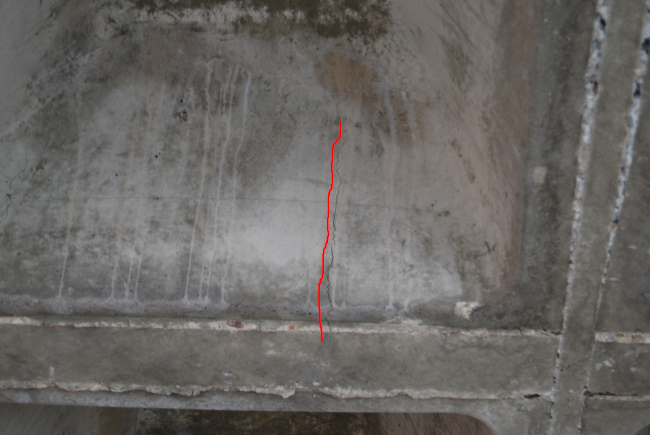
\includegraphics[width=\textwidth]{figures/DSC_0086}
  \caption{Fisuras observadas en el forjado de planta cubierta, en el encuentro de los nervios del reticular con los ábacos de menor longitud en el sentido de la luz principal}
  \end{subfigure}
\hfill
  \begin{subfigure}[r]{0.3\textwidth}
  \centering
  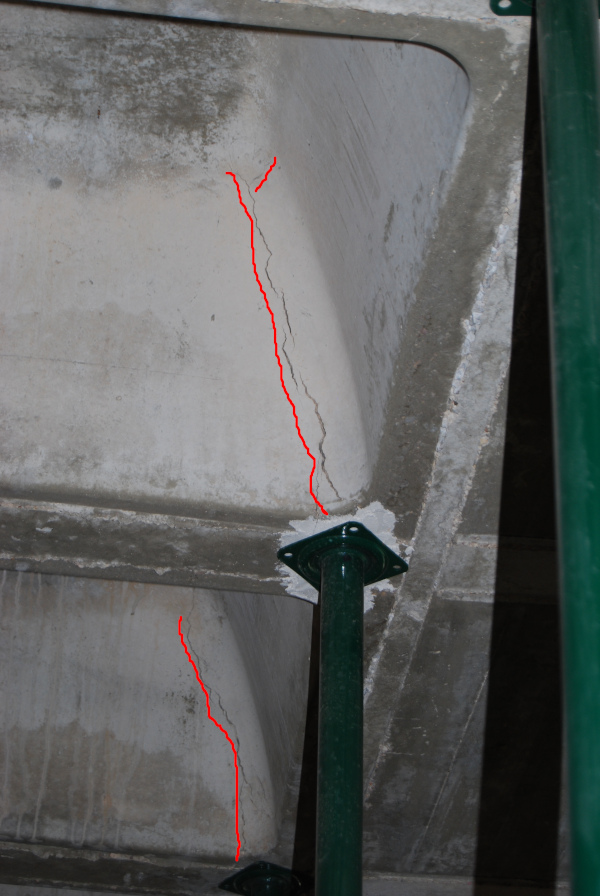
\includegraphics[width=\textwidth]{figures/DSC_0101}
  \caption{Fisuras observadas en el forjado de planta cubierta, en el encuentro de los nervios del reticular con los ábacos de mayor longitud en el sentido de la luz principal}
  \end{subfigure}
  \end{figure}
  
\begin{Parallel}{\widhtLeftCol}{\widhtRightCol}
   \ParallelLText{
    Debido a la complicada relación de la propiedad con la empresa constructora, no se dispone de información relativa a la ejecución de la obra. Se realiza, por tanto, un reconocimiento de la estructura, incluyendo mediciones de flecha, detección de armadura con pachómetro y medición de resistencia del hormigón con esclerómetro.

    En paralelo, se analiza la documentación del proyecto y se efectúa un cálculo de contraste de la estructura. Se observa que gunos aspectos del armado no quedan reflejados en el proyecto de forma que no den lugar a duda. En concreto, la armadura inferior de los nervios del reticular (constituida por 2$\Phi$20 en el forjado de planta baja y por 2$\Phi$25 en el resto de forjados) aparece representada únicamente sobre respectivos detalles en los planos de replanteo de cada una de las plantas, sobre una sección transversal del nervio. No queda claro en los detalles de armado que dicha armadura debe penetrar en el ábaco y ser anclada con patilla en el extremo del forjado. 
    
    Los resultados de detección de armadura realizados con pachómetro apuntan en la dirección de que la referida inexactitud del proyecto se ha reflejado sistemáticamente en la obra ejecutada. Esto también explica la aparente paradoja de que en el lado del forjado donde los ábacos tienen mayor longitud en el sentido de la luz principal, la fisuración está mucho más desarrollada que en el lado opuesto, ya que en estas zonas la armadura de flexión positiva del nervio se habría cortado antes y, por tanto, con mayor momento positivo. Este extremo se confirma verbalmente con el técnico encargado de la obra, quien confirma que la armadura de flexión positiva de los nervios se dispuso en la forma señalada, es decir, 2$\Phi$25 en cada nervio del reticular y 1$\Phi$12 en prolongación del nervio en el ábaco, realizándose el solape mediante prolongación del $\Phi$12 hacia el nervio.
    
   }
  
   \ParallelRText{
     \emph{Due to the complicated relationship between the property and the construction company, there is no information regarding the execution of the work. Therefore, a survey of the structure is carried out, including deflection measurements, reinforcement detection with a pachometer and concrete resistance measurement with a sclerometer.}

     \emph{In parallel, the project documentation is analyzed and a contrast calculation of the structure is carried out. It is observed that some details of the reinforcement layout are not reflected in the project in such a way that they do not give rise to doubt. Specifically, the lower reinforcement of the slab ribs (consisting of 2$\Phi$20 in the ground floor slab and 2$\Phi$25 in the rest of the slabs) is only represented on a cross-section of the rib. It is not clear in the details that said reinforcement bars must penetrate the abacus and be anchored at the end of the slab.}
    
     \emph{The results of the detection of reinforcement carried out with a pachometer point in the direction that the aforementioned inaccuracy of the project has been systematically reflected in the executed work. This also explains the apparent paradox that on the side of the slab where the abacuses are longer in the direction of the main span, the cracking is much more developed than on the opposite side, since in these areas the positive bending reinforcement of the nerve would have been cut earlier and, therefore, with a greater positive moment. This end is confirmed verbally with the technician in charge of the construction work, who confirms that the positive bending reinforcement of the ribs was arranged as guessed, that is, 2$\Phi$25 in each rib of the reticular and 1$\Phi$12 in prolongation of the rib in the abacus, performing the overlap by prolonging the $\Phi$12 towards the rib.}
     }
\end{Parallel}
\begin{figure}
  \centering
  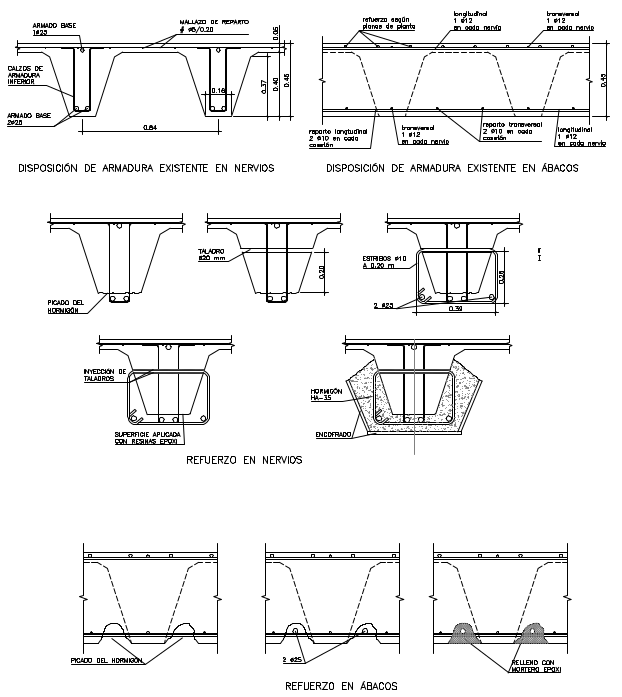
\includegraphics[width=0.8\textwidth]{figures/solucionC}
  \caption{Esquema de la solución proyectada (alternativa C)}
\end{figure}

\begin{Parallel}{\widhtLeftCol}{\widhtRightCol}
  \ParallelLText{Ante la situación de grave debilidad de la estructura, que ni siquiera es capaz de resistir con seguridad su propio peso, se realiza un estudio de soluciones de reparación, contemplando las siguientes opciones:
    
    A.- Refuerzo mediante colocación de vigas de acero bajo los forjados en cada uno de los pórticos de la estructura.

    B.- Colocación de «vigas puente» bajo el forjado de segunda planta, al disponer en esta zona de taller de un gran gálibo vertical (7,4 m).

    C.- Refuerzo mediante disposición de armadura de tracción en las zonas en que ésta resulta insuficiente.

    D.- Refuerzo mediante adhesión de bandas de fibra de carbono en la cara inferior de nervios y ábacos donde la armadura resulta insuficiente.
    
    E.- Empleo de la solución D con bandas de fibra de carbono postesadas.

    F.- Reparación mediante disposición de pilares en centro de vano en los espacios cuyo futuro uso lo permita, pretensado en el resto de pórticos y adhesión de bandas de acero al forjado.

    G.- Refuerzo de la estructura mediante postesado exterior no adherente. Esta técnica consiste en introducir, a través del tesado de cables enfundados anclados en los ábacos, momentos (y en su caso fuerzas verticales) en los forjados que son capaces de levantarlos y reducir sus tensiones de tracción.

    Esta última solución es la que se recomienda en el estudio de soluciones, al ser la que ofrece mayores garantıías de seguridad estructural durante la ejecución de la obra y en el uso futuro de las instalaciones. Por otro lado, es la única de las analizadas, junto con la solución de refuerzo con fibra postesada, capaz de corregir las deformaciones que ya ha adquirido y evitar que al recibir toda la carga desarrolle flechas por encima de los valores admisibles en la normativa española. Estas dos soluciones son también las que mantienen la diafanidad con la que inicialmente se diseñó el edificio. Frente a la solución de fibras postesadas ofrece las ventajas de menor coste y mayor seguridad en caso de incendio.

    La elección final del método de refuerzo estructural a emplear se llevó a cabo por parte de la propiedad en base a criterios económicos. Se desarrolló, por tanto, el proyecto constructivo de la solución C, permitiendo en un futuro emprender una nueva intervención basada en el empleo de armadura postesa, si se desea corregir la deformación excesiva de los forjados.
    
  }
  
  \ParallelRText{\emph{Given the serious weakness of the structure, which is not even capable of safely resisting its own weight, a study of repair solutions is carried out, analyzing the following options:}
    
     \emph{A.- Strengthening by placing steel beams under the floors in each of the frames of the structure.}

     \emph{B.- Placement of “bridge beams” under the second-floor slab, since there is a large vertical gauge (7.4 m) in this workshop area.}

     \emph{C.- Strengthening by providing tensile reinforcement bars in areas where it is insufficient.}

     \emph{D.- Adhesion of carbon fiber laminates on the underside of ribs and abacuses where the reinforcement is insufficient.}
    
     \emph{E.- Use of solution D with post-tensioned carbon fiber sheets.}

     \emph{F.- Repair by arrangement of pillars in the center of the span in spaces whose future use allows it, pre-stressing in the rest of the frames and adhesion of steel plates to the framework.}

     \emph{G.- Reinforcement of the structure by non-adherent external post-tensioning. This technique consists of introducing, through the tensioning of sheathed cables anchored in the abacuses, moments (and where appropriate vertical forces) in the slabs that are capable of lifting them and reducing their tensile stresses.}

     \emph{This last solution is the one recommended in the study of solutions, as it offers the greatest guarantees of structural safety during the execution of the work and in the future use of the facilities. On the other hand, it is the only one of those analyzed, together with the post-stressed fiber reinforcement solution, capable of correcting the deformations that it has already acquired and preventing it from developing deflections above the admissible values in Spanish regulations when receiving the full load.  These two solutions are also the ones that maintain the diaphanous spaces with which the building was initially designed. Compared to the post-tensioned fiber solution, external post-tensioning offers the advantages of lower cost and greater safety in case of fire.}

     \emph{The final choice of the structural-strengthening method was carried out by the property based on economic criteria. Therefore, the constructive project of solution C was developed, allowing the future to undertake a new intervention based on the use of external post-tensioning, if excessive deformation of the slabs is to be rectified.}
     }

  \end{Parallel}
\end{document} 
